%\paragraph{$R_0$ definition}
%\paragraph{No  vaccine reproductive number}
%\paragraph{Vaccine reproductive number}
%\paragraph{Efficacy, coverage and vaccination rate}
%
The basic reproductive number, which is generally denoted by $ R_0 $,
is a threshold quantity with which we can use
particular control strategies. The epidemiological interpretation of
$ R_0 $ is the average number of secondary cases produced by an infected
individual introduced into a population of susceptible individuals.
Using Van DenDrishe's \cite{Van2002} definition of reproductive
number we obtain
\begin{equation*}
    \label{eqn:reproductive_number}
    \begin{aligned}
        R_0 :=
        &
        \frac{\kappa}{(\kappa + \mu)(\delta_L + \mu)}
        \left(
        \mu R_1 + \delta_L
        \right)
        \left[
        \frac{p\beta_S}{R_2}
        +\frac{(1 - p) \beta_A}{\gamma_A+\mu}
        \right],
        \\
        \text{where} &
        \\
        R_1 &= 1 - \theta(1 - \epsilon),
        \\
        R_2 &= \mu + \delta_H + \gamma_S + \mu_{I_{S}}.
    \end{aligned}
\end{equation*}

The factor $\frac{p\beta_S}{R_2}$ measures the proportion of new infections
generated by a symptomatic infectious individual in the time that it lasts
infected. In a similar way, the factor $\frac{(1 - p) \beta_A}{\gamma_A+\mu}$
measures the new infections generated by an asymptomatic infectious individual
in the time that it lasts infected. The factor
$\frac{\mu R_1 + \delta_L}{\delta_L + \mu}$ measures the number
of individuals in lockdown that leave the lockdown, which can be infected.
And finally, the factor $\frac{\kappa}{\kappa + \mu}$ measures
the time of the disease's incubation.
%
If we consider that there is no lockdown, we have that $ R_0 $ is reduced to
\begin{equation*}
    \label{eqn:reproductive_number}
    \begin{aligned}
        \tilde{R}_0 :=
        &
        \frac{\kappa}{(\kappa + \mu)}
        \left[
        \frac{p\beta_S}{R_2}
        +\frac{(1 - p) \beta_A}{\gamma_A+\mu}
        \right].
    \end{aligned}
\end{equation*}
%
Note that we have the relation $ R_0 \leq \tilde{R}_0 $. These indicate that
there is greater transmission of the disease if there is no lockdown.

Considering assumptions 2, we can establish a vaccine reproductive number,
in which individuals who have already been vaccinated
can become infected individuals by being in contact with the
symptomatic infected. Using Van den Driessche’s \cite{VandenDriessche2017a}
definition of reproductive number and \cite{Alexander2004}, we obtain

\begin{equation*}
    R_{0}^V := \left[ 1-\frac{\varepsilon \lambda_V}
    {\mu+\lambda_V+\delta_V}
    -\frac{\theta\mu(1-\epsilon)}{\mu+\delta_L+\lambda_V}\right]
    (\mu R_1+\delta_L)R_0.
\end{equation*}
%
The threshold quantity $R_0^V$ is the reproductive number of infection
which can be interpreted as the number of infected people produced
by one infected individual introduced into the population in the
presence of vaccination.

\Cref{fig:rvcontour1}, displays the contour curves for $ R_0^V $ as function
of the efficacy of the vaccine $ (\epsilon) $ and of the vaccination rate $
(\lambda_V) $,
considering an immunity period induced by the vaccine of half year . Orange
line, correspond to the values of $\lambda_{Vbase}$. With this vaccination
rate, no matter how effective the vaccine is, it is not possible
to reduce the value of $R_0^V$ below one. Black line illustrate a scenario in
which we can drive the $R_0^V$  below one, considering a vaccine
efficacy of \num{0.2} and a  vaccination rate of \num{0.7}.
Here, we stress that lockdown allows the implementation of lower vaccine
efficacies to mitigate spread.
In contrast \Cref{fig:Nolockdown} displays  plausible
combinations of $\epsilon$ and $\lambda_V$ values
in order to reduce the value of $R_V$ below one. Note that in this case
we require vaccine efficacy of \SI{60}{\percent} or more and
adequate vaccination rate to drive $R_0^V$ bellow one.




\begin{figure*}[tbh]
    \centering
      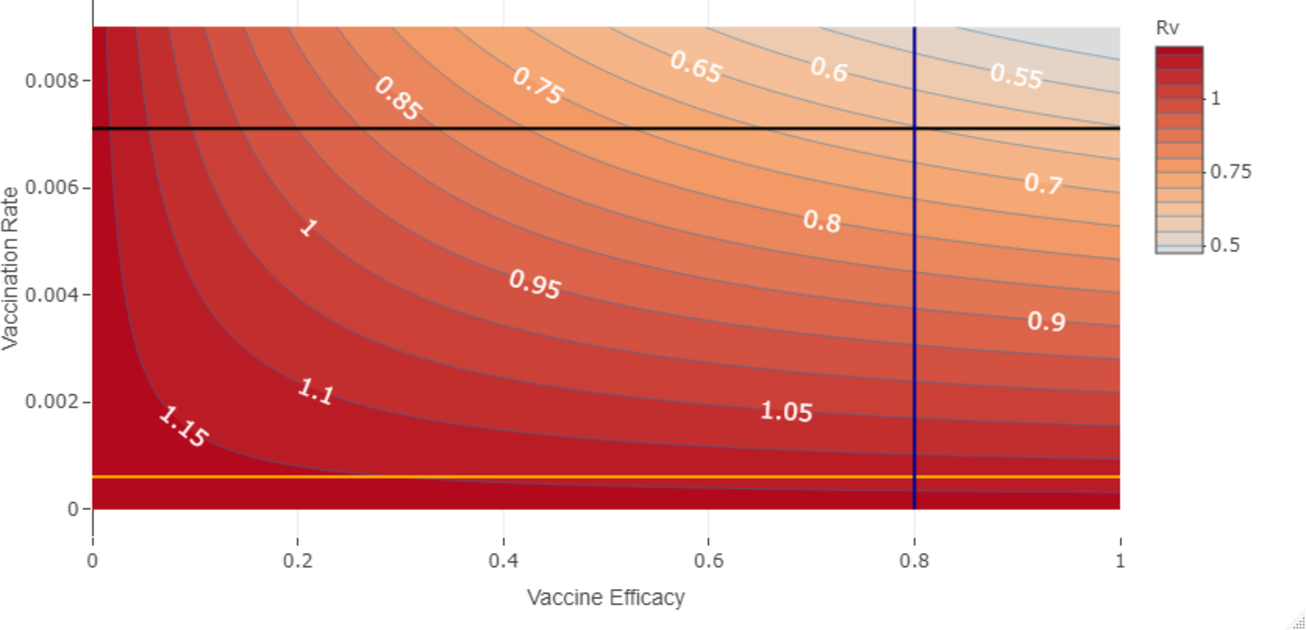
\includegraphics[scale=0.5, keepaspectratio]{Figures/Rv_contour}
    \caption{R not contour plot as function of efficacy and vaccination rate.}
    \label{fig:rvcontour1}
\end{figure*}

\begin{figure*}[tbh]
    \centering
    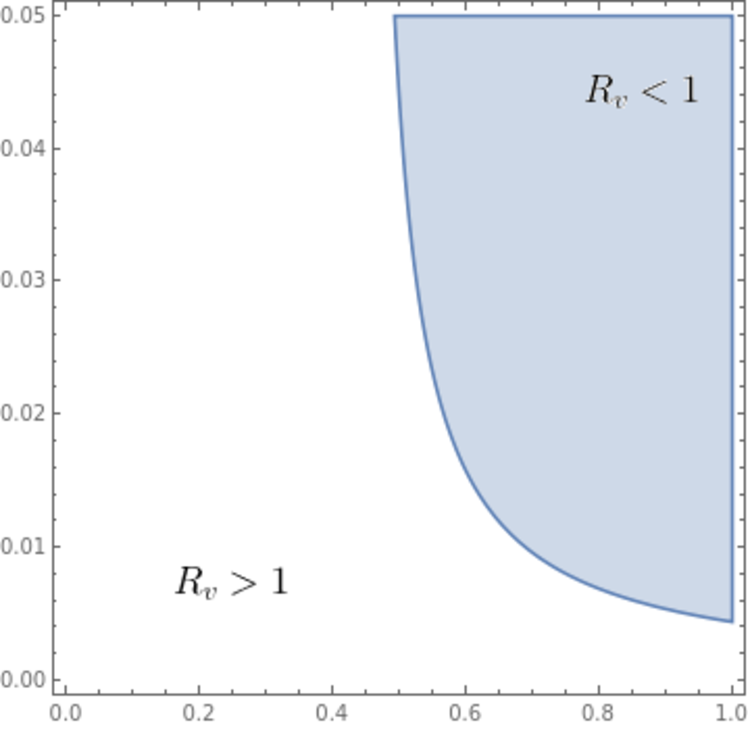
\includegraphics[scale=0.5,
    keepaspectratio]{Figures/NoLockdown.pdf}
    \caption{No lockdown Region $R_v<1$.
        \href{https://plotly.com/~AdrianSalcedo/52/}{%
            https://plotly.com/~AdrianSalcedo/52/}
    }
    \label{fig:Nolockdown}
\end{figure*}

